\documentclass[conference]{IEEEtran}

\usepackage[T1]{fontenc}
\usepackage[utf8]{inputenc}
\usepackage{amsmath}
\usepackage{booktabs}
\usepackage{cite}
\usepackage{graphicx}
\usepackage{hyperref}
\usepackage{listings}
\usepackage{pgfplots}
\usepackage{tikz}

\pgfplotsset{compat=1.18}
\usetikzlibrary{arrows.meta,positioning,shapes.geometric}

\title{Recursive Huffman Compression: An Experimental Systems Study}

\author{
\IEEEauthorblockN{Hz Project}
\IEEEauthorblockA{Reference Swift implementation and benchmark suite}
}

\begin{document}

\maketitle

\begin{abstract}
Huffman coding is normally applied once: an implementation counts symbols, builds a prefix code, emits a compressed bitstream, and stops. This paper investigates a simple question: what happens if Huffman compression is recursively applied to its own archive output? We present a modular Swift implementation of recursive Huffman archives, a versioned \texttt{.hz} container format, recursive decompression, adaptive stopping, forced-depth benchmarking, and reproducible benchmark tooling. The purpose is not to propose recursive Huffman coding as a replacement for modern compressors. Instead, we treat it as a systems experiment that exposes how Huffman coding behaves when its own metadata and encoded payload become the next input stream. Across deterministic workloads in the repository benchmark suite, most inputs stopped after one accepted Huffman layer, while highly repetitive inputs benefited from two or three accepted layers before archive overhead and increasing entropy reversed the gain. All reported measurements are produced by the repository benchmark runner and are verified by recursive decompression.
\end{abstract}

\section{Introduction}

Huffman coding is one of the standard examples of entropy coding. Given symbol frequencies, it constructs a prefix code that assigns shorter codewords to more frequent symbols and longer codewords to less frequent symbols \cite{huffman1952method}. Practical file compressors usually combine entropy coding with modeling or dictionary transforms, but a standalone Huffman implementation remains useful because it is compact, deterministic, and easy to inspect \cite{sayood2017introduction}.

Most Huffman implementations perform exactly one encoding pass. This is the natural design: after the first pass, the output is a packed bitstream plus metadata, and a good entropy coder should reduce the exploitable regularity of the original stream. A second pass is therefore expected to have little opportunity to improve the result, and may instead add archive overhead.

This work asks a deliberately narrow question: \emph{what happens if Huffman compression is recursively applied to its own output?} We answer it by extending the Hz Swift/SwiftUI repository with a clean reference compression engine, recursive archive metadata, full and partial recursive decompression, and a benchmark suite that records every attempted compression layer. The SwiftUI application remains a frontend over a compression service, while the compression engine is isolated behind a small protocol so that a future native implementation can replace it through a stable interface.

The contributions are:
\begin{itemize}
    \item a modular Swift Huffman implementation split into frequency counting, tree construction, bit reading and writing, archive serialization, and engine orchestration;
    \item a versioned \texttt{.hz} archive format that records original byte count, encoded bit count, frequency metadata, payload bytes, flags, and recursive layer count;
    \item adaptive recursive compression that accepts only strictly smaller archive layers and discards the first non-improving candidate;
    \item recursive decompression that unwraps exactly the recorded number of layers, with support for partial decompression;
    \item forced-depth benchmarking for studying compression trajectories beyond the adaptive stopping point;
    \item deterministic workloads, CSV outputs, analysis tooling, and verification by round-trip decompression.
\end{itemize}

\section{Background}

Huffman coding constructs an optimal prefix code for a known set of symbol frequencies under the standard symbol-by-symbol coding model \cite{huffman1952method}. For byte-oriented files, the encoder counts byte frequencies, builds a binary tree whose leaves are byte values, derives a variable-length code for each byte, and writes the corresponding bits to the output. The decoder rebuilds the same tree from transmitted metadata and traverses it bit by bit until the original symbols are recovered.

A standalone Huffman archive must store more than the compressed payload. It needs enough metadata to reconstruct the code and enough length information to distinguish meaningful encoded bits from padding bits in the final byte. Without the original byte count or encoded bit count, a decoder may incorrectly interpret padding as real data. The Hz archive format therefore stores both values.

Recursive Huffman compression is expected to show diminishing returns for two reasons. First, a Huffman-coded payload should be closer to a high-entropy byte stream than the original input, especially for ordinary text. Second, each archive layer carries metadata: magic bytes, version fields, length fields, frequency entries, and a payload boundary. A subsequent layer must overcome this overhead before it can improve total file size.

\section{Recursive Huffman Compression}

Let $x_0$ be the original byte sequence. A single Huffman archive layer computes $x_1 = H(x_0)$, where $H$ is the archive-producing Huffman encoder. Recursive Huffman compression repeats this process:
\[
    x_{i+1} = H(x_i).
\]
Layer 1 is the ordinary archive produced from the original input. Layer 2 is an archive whose input is the complete Layer 1 archive, including its header and payload. The process may continue either until a configured forced depth is reached or until an adaptive stopping rule rejects the next layer.

The adaptive rule used by Hz is intentionally conservative. The first layer is accepted so that the output is always an archive. Each additional candidate layer is accepted only if its total archive size is strictly smaller than the current accepted archive. If a candidate is equal in size or larger, that candidate is discarded and the previous archive remains the result.

\begin{figure}[t]
\centering
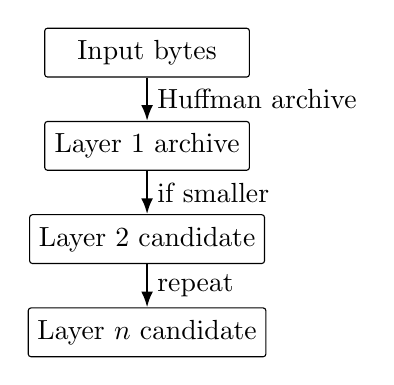
\begin{tikzpicture}[
    node distance=0.55cm,
    box/.style={draw, rounded corners=1pt, minimum width=2.6cm, minimum height=0.62cm, align=center},
    arrow/.style={-{Latex[length=2mm]}, thick}
]
\node[box] (input) {Input bytes};
\node[box, below=of input] (l1) {Layer 1 archive};
\node[box, below=of l1] (l2) {Layer 2 candidate};
\node[box, below=of l2] (ln) {Layer $n$ candidate};
\draw[arrow] (input) -- node[right]{Huffman archive} (l1);
\draw[arrow] (l1) -- node[right]{if smaller} (l2);
\draw[arrow] (l2) -- node[right]{repeat} (ln);
\end{tikzpicture}
\caption{Recursive Huffman compression treats the entire previous archive as the next input stream.}
\label{fig:nesting}
\end{figure}

\begin{lstlisting}[language={},caption={Adaptive recursive compression.},label={alg:adaptive},basicstyle=\ttfamily\footnotesize,frame=single]
best = HuffmanArchive(input)
layers = 1

while layers <= maximumAdditionalDepth:
    candidate = HuffmanArchive(best)
    if size(candidate) >= size(best):
        break
    best = candidate
    layers += 1

return withRecursiveLayerCount(best, layers)
\end{lstlisting}

Forced-depth mode disables the adaptive size check and records all attempted layers up to a configured maximum. It is useful for experiments because it reveals whether size reduction continues, plateaus, or reverses after the adaptive rule would normally stop. The production file workflow uses adaptive mode.

\section{Archive Format}

Hz archives use a binary \texttt{.hz} format. The current version is version 2 and is documented in the Swift implementation. All multi-byte integer fields are little-endian. The layout is shown in Fig.~\ref{fig:archive-layout}.

\begin{figure}[t]
\centering
\resizebox{\columnwidth}{!}{%
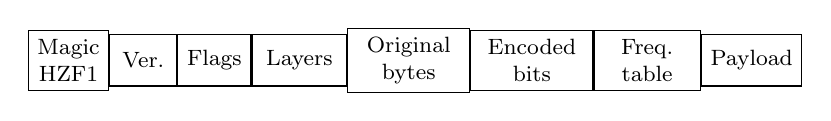
\begin{tikzpicture}[
    field/.style={draw, minimum height=0.65cm, align=center},
    every node/.style={font=\footnotesize}
]
\node[field, minimum width=1.0cm] (magic) {Magic\\HZF1};
\node[field, minimum width=0.85cm, right=0cm of magic] (version) {Ver.};
\node[field, minimum width=0.75cm, right=0cm of version] (flags) {Flags};
\node[field, minimum width=1.2cm, right=0cm of flags] (layers) {Layers};
\node[field, minimum width=1.55cm, right=0cm of layers] (orig) {Original\\bytes};
\node[field, minimum width=1.55cm, right=0cm of orig] (bits) {Encoded\\bits};
\node[field, minimum width=1.35cm, right=0cm of bits] (freqs) {Freq.\\table};
\node[field, minimum width=1.25cm, right=0cm of freqs] (payload) {Payload};
\end{tikzpicture}
}
\caption{Version 2 \texttt{.hz} archive layout. The encoded bit count prevents padding bits from being decoded as symbols.}
\label{fig:archive-layout}
\end{figure}

The recursive layer count is stored only in the outermost final archive. Inner layers write a count of zero, which means that the archive does not advertise a total recursion depth. This choice keeps inner archives independently decodable as ordinary Huffman archives while letting a complete recursive archive declare how many layers must be removed to recover the original data.

Full decompression reads the outermost layer count and unwraps exactly that many Huffman layers. Partial decompression removes a caller-specified number of outer layers and returns the remaining valid \texttt{.hz} archive. The decoder never relies on padding bits for termination: it stops after the recorded original byte count and rejects archives whose headers or payloads are truncated or inconsistent.

\section{Benchmark Methodology}

The benchmark suite is implemented in \texttt{benchmarks/run.sh} and \texttt{benchmarks/Sources/main.swift}. The runner compiles the production Swift engine with optimization and executes it on deterministic workloads. If no workload directory is supplied, the benchmark program generates its own workloads under \texttt{benchmarks/workloads/generated}. This avoids dependence on external corpora and makes the reported measurements reproducible from the repository.

The committed measurements use five generated workloads:
\begin{itemize}
    \item \textbf{high-entropy}: deterministic pseudorandom bytes;
    \item \textbf{compressed-like}: bytes intended to resemble already compressed data;
    \item \textbf{ordinary-prose}: repeated natural-language-like text;
    \item \textbf{repetitive-text}: highly repetitive textual data;
    \item \textbf{single-byte}: a degenerate stream containing one repeated byte.
\end{itemize}

For each workload, the runner records original size, output size for every attempted pass, accepted layer count, best pass, stopping reason, compression time, decompression time, platform string, and verification status. Verification decompresses the produced archive and compares the bytes with the original input. The runner writes per-pass and summary CSV files. The paper tables and plot data are generated from the CSV snapshots in \texttt{papers/recursive-huffman/artifacts/data} by \texttt{papers/recursive-huffman/scripts/generate\_artifacts.py}.

\section{Results}

\begin{table}[t]
\caption{Adaptive recursive Huffman results. ``Baseline'' is one Huffman archive layer.}
\label{tab:results}
\centering
\scriptsize
\begin{tabular*}{\columnwidth}{@{\extracolsep{\fill}}lrrrrrr@{}}
\toprule
Workload & In & 1-pass & Adapt. & L & Ratio & $\Delta$ \\
\midrule
Compressed-like & 16,384 & 18,574 & 18,574 & 1 & 1.134 & +13.4\% \\
High entropy & 16,384 & 18,714 & 18,714 & 1 & 1.142 & +14.2\% \\
Ordinary prose & 22,960 & 12,786 & 12,786 & 1 & 0.557 & -44.3\% \\
Repetitive text & 13,312 & 4,432 & 2,325 & 2 & 0.175 & -82.5\% \\
Single byte & 16,384 & 2,083 & 293 & 3 & 0.018 & -98.2\% \\
\bottomrule
\end{tabular*}
\end{table}


Table~\ref{tab:results} reports the adaptive results. The high-entropy and compressed-like workloads grew after one Huffman archive layer. This is expected: their byte distributions do not provide enough exploitable skew to offset archive metadata. Ordinary prose compressed substantially in one layer, but the next attempted layer was larger, so adaptive mode stopped at the baseline archive.

The highly repetitive workloads behaved differently. Repetitive text improved from 4,432 bytes after one layer to 2,325 bytes after two accepted layers. The single-byte workload improved from 2,083 bytes after one layer to 371 bytes after two layers and 293 bytes after three layers. In both cases, the next attempted layer grew and was rejected.

\begin{table}[t]
\caption{Compression trajectory for adaptive mode. Rejected rows are attempted layers that were discarded by the stopping rule.}
\label{tab:passes}
\centering
\small
\begin{tabular}{lrrrrr}
\toprule
Workload & Pass & Input & Output & Ratio & Accepted \\
\midrule
Compressed-like & 1 & 16,384 & 18,574 & 1.134 & yes \\
Compressed-like & 2 & 18,574 & 20,159 & 1.085 & no \\
High entropy & 1 & 16,384 & 18,714 & 1.142 & yes \\
High entropy & 2 & 18,714 & 20,318 & 1.086 & no \\
Ordinary prose & 1 & 22,960 & 12,786 & 0.557 & yes \\
Ordinary prose & 2 & 12,786 & 14,773 & 1.155 & no \\
Repetitive text & 1 & 13,312 & 4,432 & 0.333 & yes \\
Repetitive text & 2 & 4,432 & 2,325 & 0.525 & yes \\
Repetitive text & 3 & 2,325 & 2,732 & 1.175 & no \\
Single byte & 1 & 16,384 & 2,083 & 0.127 & yes \\
Single byte & 2 & 2,083 & 371 & 0.178 & yes \\
Single byte & 3 & 371 & 293 & 0.790 & yes \\
Single byte & 4 & 293 & 607 & 2.072 & no \\
\bottomrule
\end{tabular}
\end{table}


\begin{figure}[t]
\centering
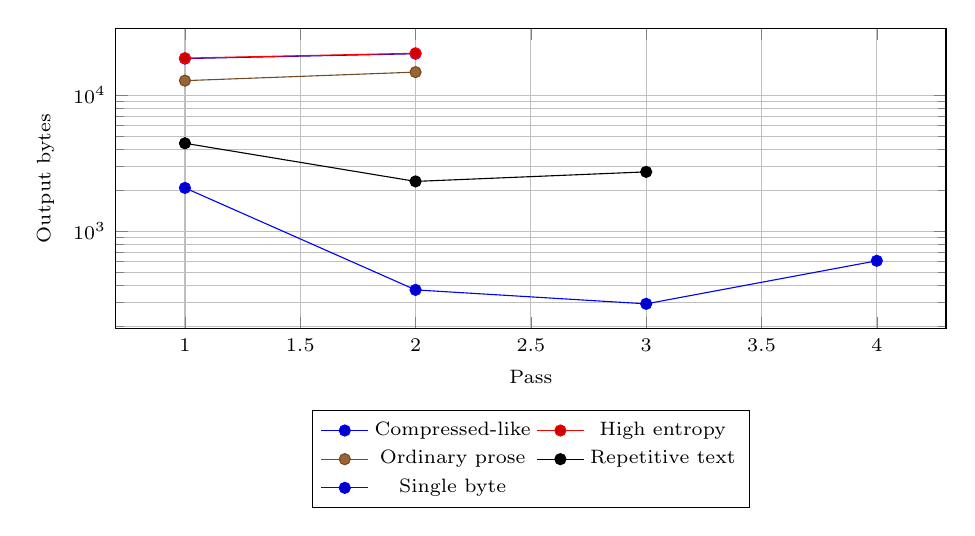
\begin{tikzpicture}
\begin{axis}[
    width=\columnwidth,
    height=5.4cm,
    xlabel={Pass},
    ylabel={Output bytes},
    ymode=log,
    grid=both,
    legend style={font=\scriptsize, at={(0.5,-0.27)}, anchor=north, legend columns=2},
    tick label style={font=\scriptsize},
    label style={font=\scriptsize}
]
\addplot+[mark=*] coordinates {(1,18574) (2,20159)};
\addlegendentry{Compressed-like}
\addplot+[mark=*] coordinates {(1,18714) (2,20318)};
\addlegendentry{High entropy}
\addplot+[mark=*] coordinates {(1,12786) (2,14773)};
\addlegendentry{Ordinary prose}
\addplot+[mark=*] coordinates {(1,4432) (2,2325) (3,2732)};
\addlegendentry{Repetitive text}
\addplot+[mark=*] coordinates {(1,2083) (2,371) (3,293) (4,607)};
\addlegendentry{Single byte}
\end{axis}
\end{tikzpicture}

\caption{Adaptive compression trajectory over all attempted passes. The y-axis is logarithmic; individual workload values are listed in Table~\ref{tab:passes}.}
\label{fig:trajectory}
\end{figure}

Table~\ref{tab:passes} shows why adaptive stopping is important. Every workload eventually produced a non-improving candidate. The rejected pass is not part of the final archive. This distinction matters because a naive recursive compressor that blindly applies a fixed number of layers would make several of these outputs larger than the best accepted archive.

All rows in the committed benchmark summaries report successful verification. The benchmark runner verifies each final archive by recursive decompression, so the reported sizes are tied to decodable outputs rather than encoder-only measurements.

\section{Discussion}

The measurements support a conservative interpretation. Recursive Huffman compression is not a general-purpose improvement over ordinary Huffman coding. For high-entropy and already-compressed-like data, one archive layer already increases size. For ordinary prose, the first Huffman pass captures much of the available byte-frequency skew, and the second pass loses to metadata overhead. These outcomes match the expectation that entropy coding tends to remove the very regularity that a subsequent entropy-coding pass would need.

The interesting cases are the pathological or highly repetitive inputs. A single repeated byte creates a very small code alphabet and a structured archive. The next Huffman layer can exploit the byte distribution of that archive representation, not merely the original data. This explains why the single-byte workload can improve for several layers even though a practical compressor would normally use a run-length or dictionary transform before entropy coding.

Archive overhead is central to the result. Every recursive layer stores magic bytes, version fields, counts, a frequency table, and a payload. Adaptive stopping prevents the final output from including a candidate that fails to overcome this overhead. It does not make recursive Huffman free: the encoder still spends time constructing and testing the rejected layer. The measured workloads are small, so the timing values should be treated as implementation measurements for this repository rather than broad performance claims.

The system architecture is also part of the contribution. The SwiftUI application calls a file compression service, which calls a \texttt{CompressionEngine}. The current implementation is \texttt{SwiftHuffmanEngine}. This boundary is intentionally narrow: a future C, C++, Rust, or Zig engine can expose a C ABI and preserve the same high-level behavior.

\section{Limitations}

The benchmark suite uses deterministic generated workloads rather than a large public corpus. This makes the results reproducible from the repository, but it limits external validity. The implementation is a Swift reference engine, not a tuned native compressor. Timing results include the behavior of this implementation and should not be compared directly with mature compression libraries.

The recursive archive format is intentionally simple. It stores enough metadata for safe decompression and partial unwrapping, but it is not optimized for minimum header size. The current adaptive stopping rule considers total archive bytes only. Other criteria, such as time budgets, estimated entropy, payload-only deltas, or application-specific thresholds, may produce different stopping decisions.

\section{Future Work}

The next engineering step is to replace the Swift reference engine with a native implementation behind the existing compression engine interface. Rust, C, C++, and Zig are all plausible candidates if exposed through a stable C ABI. Streaming compression is another natural extension: the current design operates on complete \texttt{Data} values, which is convenient for a reference implementation but unsuitable for large files.

Several experimental directions are also open. Recursive behavior could be compared against arithmetic coding, asymmetric numeral systems, or Huffman coding preceded by simple transforms. The benchmark suite could add public corpora, larger binary inputs, and multiple stopping criteria. Forced-depth mode already provides the mechanism needed to study such trajectories without changing the application workflow.

\section{Conclusion}

This paper presented recursive Huffman compression as an experimental systems study. The Hz repository now contains a modular Swift reference implementation, a safer versioned archive format, adaptive and forced recursive compression modes, recursive decompression, benchmark tooling, and generated workloads. The measured results are modest but informative: most workloads stop after one accepted layer, while highly repetitive inputs can improve across multiple recursive layers before archive overhead dominates. Adaptive stopping is therefore essential. Recursive Huffman is best understood not as a replacement for modern compressors, but as a compact experiment in how entropy-coded archives behave when they become their own input.

\bibliographystyle{IEEEtran}
\bibliography{references}

\end{document}
